\subsection{Degree distribution}
Figure \ref{fig:degree-distribution} shows the complementary cumulative distribution function (CCDF) of the proportion of nodes whose degree is larger than the given degree.
\begin{figure}
\centering
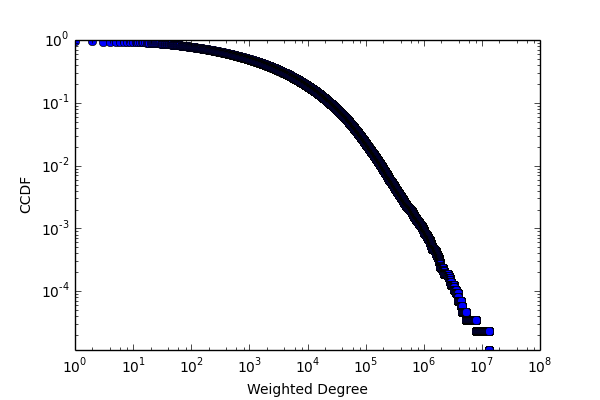
\includegraphics[scale=0.5]{../weighted_degree_ccdf.png}
\caption{CCDF of weighted degree in $\mathcal{G}$}
\label{fig:degree-distribution}
\end{figure}
As stated previously, the weight of an edge is an inverse of the distance between venues, which represent the strength of association between two venues. Then weighted degree is how strongly a venue is associated with all the other venues, therefore shows the relevance of a venue. The power law behaviour seen as the straight line in Figure \ref{fig:degree-distribution} shows that the relevance of venues is largely heterogeneous and could be explained by rich-get-richer model. Indeed, it is perfectly plausible that the higher the relevance of a venue is, the more people visit the location.

One may say that the total number of check-in represents the popularity of a venue. Expectedly, this also exhibits the power law distribution as can be seen in Figure \ref{fig:checkin-distribution}, which is CCDF of the proportion of nodes whose total check-in count is larger than the given count.
\begin{figure}
\centering
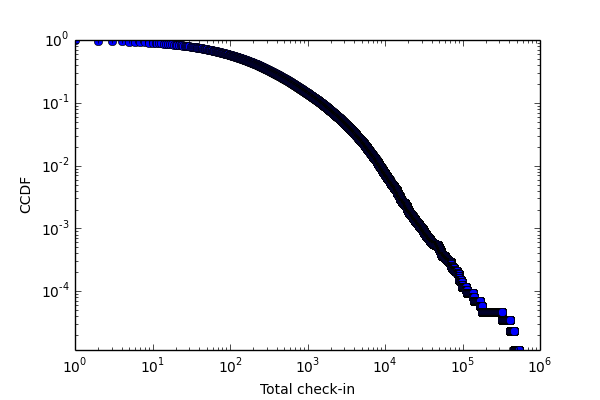
\includegraphics[scale=0.5]{../checkin_new_ccdf.png}
\caption{CCDF of total check-in counts in $\mathcal{G}$}
\label{fig:checkin-distribution}
\end{figure}

Relevance and popularity seems to be two concepts that could be related somehow. Unfortunately the data says otherwise. Each point in Figure \ref{fig:rel-pop} and Figure \ref{fig:rel-pop-zoomed-in} represents a venue in Foursquare dataset, where the latter only shows the venue with fewer than 5000 check-ins. There does not seem to be any clear correlation between two metrics.

\begin{figure}
\centering
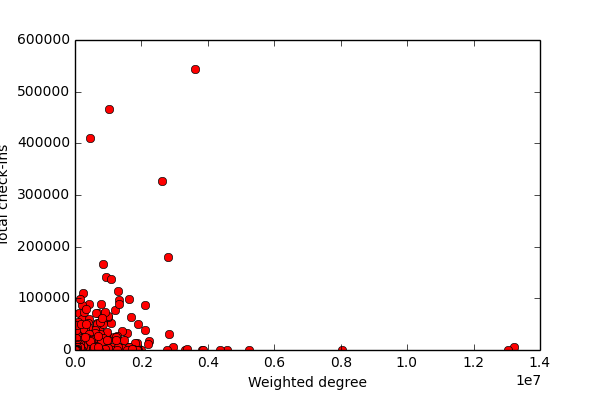
\includegraphics[scale=0.5]{../rel_pop.png}
\caption{Relation between weighted degree and total check-in counts}
\label{fig:rel-pop}
\end{figure}
\begin{figure}
\centering
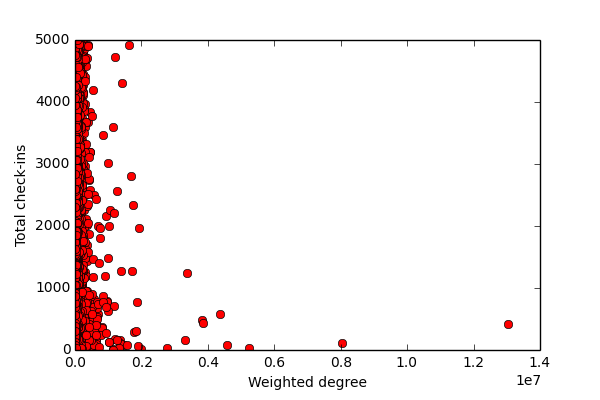
\includegraphics[scale=0.5]{../rel_pop_5000.png}
\caption{Relation between weighted degree and total check-in counts for venues with fewer than 5000 check-ins}
\label{fig:rel-pop-zoomed-in}
\end{figure}

\subsection{Weight distribution}
Recall that we defined the weight of the edge to be an inverse of the distance between two nodes which it connects.
Since distance is much more intuitive metric to consider, we look at the distribution of the inverse of the weight (i.e. distance) in this section.
Figure \ref{fig:distance-ccdf} shows the CCDF of the proportion of nodes whose distance is larger than the given distance, and Figure \ref{fig:distance-distribution} shows the frequency distribution of the distance.
\color{red} We can interpreted these graphs to show the relationship between the distance and the likeliness of checking in. \color{black}
Unlike the total check-in counts or the degree which follows the power law distribution, it shows an exponential distribution with a faster decaying tail.
This is perhaps due to the fact that the check-ins in the dataset are limited to ones in New York, which imposes an upper limit.
\begin{figure}
\centering
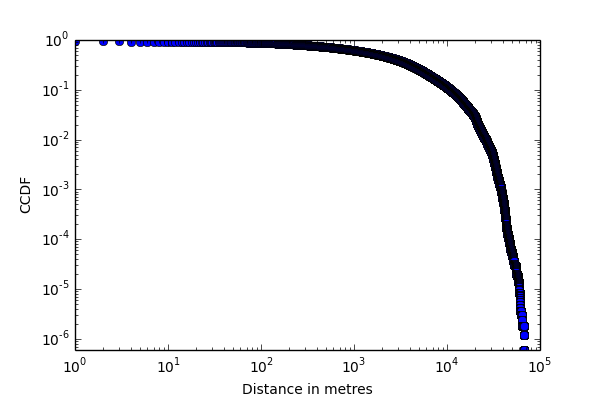
\includegraphics[scale=0.5]{../distance_metres_ccdf.png}
\caption{CCDF of the distance of the transition}
\label{fig:distance-ccdf}
\end{figure}
\begin{figure}
\centering
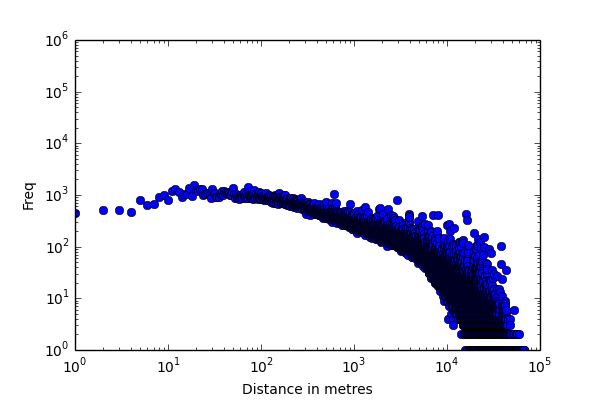
\includegraphics[scale=0.5]{../distance_metres_distribution.png}
\caption{Distribution of the distance of the transition}
\label{fig:distance-distribution}
\end{figure}
\subsection{Clustering Coefficient}
A generalised clustering coefficient for weighted graph was prorposed by \cite{saramaki2007generalizations}. A weighted graph can be translated into a fully connected graph, where the edge that does not exist in the original graph bear zero weight. This gives the notion of \emph{intensity} of a subgraph $g$ with a set of edges $e_{g}$ and a set of nodes $n_{g}$ \citep{saramaki2007generalizations}:
\begin{align*}
I(g) = \left( \prod_{(i, j)\in e_{g}}^{}w_{i, j} \right)^{\frac{1}{|e_{g}|}}
\end{align*}
An unweighted graph can be regarded as a weighted graph where all the edges bear a constant weight therefore the intensity of any triangle is constant. This can be generalised using intensity to obtain the clustering coefficient of a node $i$ as follows\citep{saramaki2007generalizations}:
\begin{align*}
C_i = \frac{2}{(k_i(k_i-1)}\sum_{j, k}^{}(\widetilde{w}_{i, j}\widetilde{w}_{j, k}\widetilde{w}_{k, i})^{\frac{1}{3}}
\end{align*}
where $\widetilde{w}_{i, j}$ is a weight of the edge between $i$ and $j$ normalised with respect to the largest weight of a edge in the network. 
The clustering coefficient of $\mathcal{G}$ is $7.99\mathrm{e}{-5}$ which is very low. This is perhaps is because many triangles include at least one edge with very low weight, which pulls down the intensity of the triangle.
The clustering coefficient of an unweighted graph $\mathcal{G}_u$, which has the same edges and nodes as $\mathcal{G}$ is $0.135$. This is significantly higher than the clustering coefficient of an unweighted random graph $2.85\mathrm{e}{-4}$with the same number of nodes and the average degree as $\mathcal{G}_u$. The clustering coefficient of  $\mathcal{G}_u$ can be interpreted as the transitivity of the existence of association. In other words, it quantifies the extent to which venue A and C are visited in succession if venue A and B, and venue B and C are visited one after the other.
\color{red}average path length \color{black}